% !Mode:: "TeX:UTF-8:Main"
\documentclass[multi,tikz]{article}
\usepackage{geometry}
\geometry{margin=1pt,paperwidth=35.5cm,paperheight=4.5cm}
\usepackage[svgnames,x11names]{xcolor}
\definecolor{basecolour}{RGB}{0,128,128}
\definecolor{myblue}{RGB}{0,170,212}
\definecolor{mygreen}{RGB}{55,200,113}
\usepackage{tikz}
\usetikzlibrary{tikzlings}
\usetikzlibrary{ducks}
\newcounter{steps}
\newcommand\tagpost[2][xshift=-26,yshift=-7]{%
 \stepcounter{steps} %\showthe\value{steps}\show
 \ifnum\the\value{steps}<\the\value{page}
\begin{scope}[#1]
  \fill[brown!50!black, rounded corners=1, rotate=-20] (0.8,-0.25) rectangle (0.9,1.75);
  %\fill[green, rounded corners=1, rotate=-20] 
  %  (0.4,1.7) rectangle (1.3,2.4);
  %\fill[blue, rounded corners=1, rotate=-20] (0.45,1.75) rectangle (1.25,2.35);
   \node[draw=myblue,very thick,rounded corners=1,fill=basecolour!80!white,rotate=-20,font=\bfseries\sffamily,text=white
    ] at (1.37,1.25) {#2};
   \end{scope}
 \fi   
   }
\begin{document}
\foreach \x  in {1,2,...,20}{
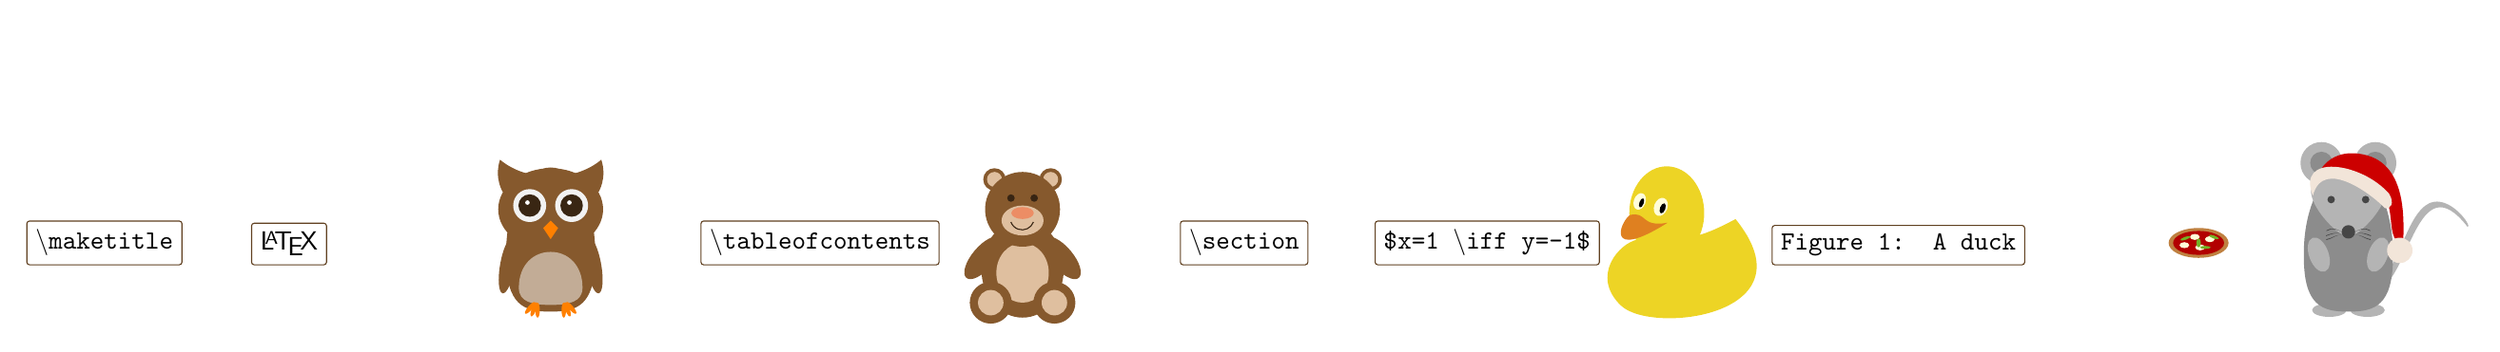
\begin{tikzpicture}
\path(0,1);
\tagpost[xshift=-3.5cm,yshift=-1.5cm]{Title}
\path (-2.5,-3)node[yshift=0.8cm,xshift=-1cm,font=\ttfamily,anchor=south west,fill=white,draw=brown!50!black, rounded corners=1]{\textbackslash maketitle};

\tagpost[xshift=-0.5cm,yshift=-1.5cm]{actualtext=LaTeX}
\path (0.5,-3)node[yshift=0.8cm,xshift=-1cm,font=\sffamily,anchor=south west,fill=white,draw=brown!50!black, rounded corners=1]{\LaTeX};

\tagpost[xshift=3cm,yshift=-1.5cm]{Figure, alt=Owl}
\path (3.5,-3)pic{owl};

\tagpost[xshift=6.5cm,yshift=-1.5cm]{TOC}
\path (6.5,-3)node[yshift=0.8cm,xshift=-1cm,font=\ttfamily,anchor=south west,fill=white,draw=brown!50!black, rounded corners=1]{\textbackslash tableofcontents};

\tagpost[xshift=9.5cm,yshift=-1.5cm]{Figure, alt=Bär}
\path (9.8,-3)pic{bear};

\tagpost[xshift=12.5cm,yshift=-1.5cm]{H1}
\path (12.5,-3)node[yshift=0.8cm,xshift=-0.6cm,font=\ttfamily,anchor=south west,fill=white,draw=brown!50!black, rounded corners=1]{\textbackslash section};

\tagpost[xshift=15.5cm,yshift=-1.5cm]{\begin{tabular}[b]{l}Formula\\ math\\ mi mo mn\end{tabular}}
\path (15.5,-3)node[yshift=0.8cm,xshift=-1cm,font=\ttfamily,anchor=south west,fill=white,draw=brown!50!black, rounded corners=1]{\$x=1 \textbackslash iff y=-1\$};

\tagpost[xshift=18.5cm,yshift=-1.5cm]{Figure, alt=Dinner}
\path (17.5,-3)pic{duck};

\tagpost[xshift=21.5cm,yshift=-1.5cm]{Caption}
\path (20.8,-3)node[yshift=0.8cm,xshift=-1cm,font=\ttfamily,anchor=south west,fill=white,draw=brown!50!black, rounded corners=1]{Figure 1: A duck};

\tagpost[xshift=24.5cm,yshift=-1.5cm]{artifact}
\path (24.5,-2.5)pic[duck/pizza,duck/invisible]{duck};


\tagpost[xshift=27.5cm,yshift=-1.5cm]{Figure, alt=Santa Claus}
\path (27.5,-3)pic[thing/santa=red!80!black]{mouse};
\end{tikzpicture}\newpage\setcounter{steps}{0}}

\end{document}
